\begin{center}
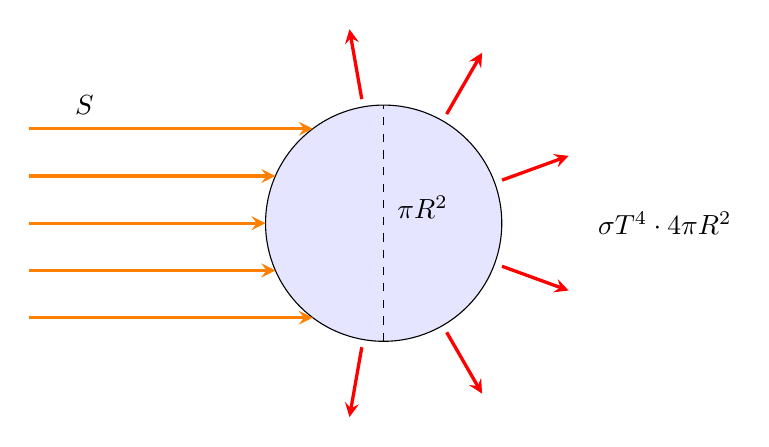
\begin{tikzpicture}[>=stealth]
 \draw[fill=blue!10] (0,0) circle (1.5);
 \foreach \y/\x in {1.2/-0.9, 0.6/-1.375, 0/-1.5, -0.6/-1.375, -1.2/-0.9} \draw[->, very thick, orange] (-4.5,\y) -- (\x,\y);
 \node[anchor=south] at (-3.8,1.25) {$S$};
 \draw[dashed] (0,-1.5) -- (0,1.5);
 \node[anchor=west] at (0.05,0.2) {$\pi R^2$};
 \foreach \a in {20,60,100,-20,-60,-100} \draw[->, very thick, red] (\a:1.6) -- (\a:2.5);
 \node[anchor=west] at (2.6,0) {$\sigma T^4\cdot 4\pi R^2$};
\end{tikzpicture}
\end{center}

Die Erde fängt mit ihrer Querschnittsfläche $\pi R^2$ die Sonnenstrahlung mit der Intensität $S = \SEO$ (Solarkonstante, FoTaBe Umschlag hinten) auf. Als schwarzer Körper absorbiert sie alles und strahlt mit ihrer ganzen Oberfläche $4\pi R^2$ wieder ab. Im Gleichgewicht gilt
\begin{align}
 S\,\pi R^2 &= \sigma\,T^4\,4\pi R^2 \\
 T &= \TEF \\
   &= \sqrt[4]{\frac{\SE}{4\cdot\sig}} \\
   &= \TE \approx \result{\TEP{0}{2}}
\end{align}
Das entspricht $\vartheta = \tEP{0}{1}$. Der Erdradius kürzt sich heraus. Dass die mittlere Oberflächentemperatur trotzdem etwa so gross ist, ist Zufall: Die Erde reflektiert rund ein Drittel der Sonnenstrahlung (Wolken, Eis), dafür hält der Treibhauseffekt der Atmosphäre die Oberfläche wärmer.
